\documentclass[10pt,conference,compsocconf]{IEEEtran}

\usepackage[hidelinks]{hyperref}
\usepackage{graphicx}	% For figure environment


\begin{document}
\title{Stochastic Gradient Quantization : \\ Saving Bandwidth in Distributed Learning}

\author{
  Cheng Soon Ong\\
  \textit{Department of Computer Science, ETH Zurich, Switzerland}
}

\maketitle

\begin{abstract}

	With the ever-increasing size of machine learning models, and with the development of scale-out architectures, distributed learning has become crucial to exploit the benefits of parallelism. Stochastic Gradient Descent (SGD) is naturally suited for this task as it can leverage the distribution of data. However, the necessary exchange of gradients among workers leads to bandwidth limitations becoming a new performance bottleneck. Quantized SGD (QSGD) addresses this issue through quantization of gradients before their exchange. This report aims to analyze the effects on convergence of such lossy compression schemes.
\end{abstract}

\section{Introduction}

[If too much space, communication costs linked to bandwidth usage and scalability issues]

ah

QSGD \cite{quant}  uses gradient quantization to trade-off lower bandwidth usage for higher variance in distributed training, and shows that models will still converge to local optima. The paper proposes two algorithmic ideas : a stochastic gradient quantization scheme and an efficient encoding of quantized gradients. In this report, we will only be concerned about the first idea and we will try to analyze the effects of gradient quantization on convergence rates in practice.

We will be presenting the training of 3 popular models in different distributed settings and quantization rates, followed by a discussion. Remarkably, we found that in our applications we can reduce bandwidth usage by at least 4x without any percieved downside, and up to 8x with minor increase on convergence time. In terms of network accuracy, quantized training converges towards each model's top accuracy, and sometimes generalizes better on the test set.

\section{Technical Background}

Quantization is a signal processing technique in which continuous values are mapped to a discrete subset of the value range. This enables values to be encoded in a space efficient manner while preserving most of the original information. This quantization can be deterministic, and map to the closest discrete value, or stochastic and map to discrete values with probability proportional to their distance, see Fig. \ref{fig:quant}. 

\begin{figure}[b]
  \centering
  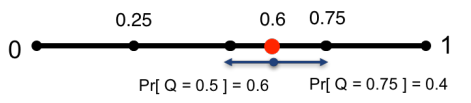
\includegraphics[scale=0.45]{quant}
  \caption{Stochastic Quantization}
  \vspace{-3mm}
  \label{fig:quant}
\end{figure}

QSGD uses stochastic quantization defined as such :

give quantization formula

Gradients can be compressed to sending a 32 bit norm, a bit vector of signs and a n element vector of q bit quantization indices.

put example of quantized vector


This compression of gradients introduces a quantization error, which we can mitigate during training with a process we will call error correction. Upon each iteration, save the quantization error, and add it to the gradient on the next iteration. This preserves even more information in expectation.


\section{Experiments}

\subsection{Model Definition}

\subsubsection{Dataset}

We will conduct our experiments on an image classification task on the CIFAR-10 dataset. It contains 60,000 colored 32x32 pixel images, with 10 differents classes. We will be using 50,000 samples for training, with a 0.1 validation split (5,000 samples), and the remaining 10,000 samples are used for testing.

\subsubsection{Models}

We train 3 popular models : AlexNet, ResNet50 and ResNet110.

Short intro to the models

We will train our models on 1, 2, 4, and 8 nodes

\subsubsection{Optimization}

As mentionned earlier, SGD is well suited for distributed learning tasks as it can take advantage of the data parallelism. We therefore split our data accross nodes, perform computation per node, and then average out the gradients. Quantization of the gradients is added at each node level before global averaging.

\subsubsection{Evaluation Method}
How do we evaluate the networks ?

Run baseline model and compare

Accuracy - do we reach top ??
Convergence time - in how many epochs (roughly)
Communication costs - speedup from quantization bits


\subsubsection{ Stochastic vs without}
\subsubsection{ Added error correction}

\subsection{Simulating Distributed Training}

Distributed training is difficult to implement properly and requires to deal with multiple GPUs, message passing protocols, gradient encodings and other problems. We decided to simulate distributed training instead, using a single GPU which sequentially computes forward and backward passes, quantizes gradients, and averages them out on a single model. We are still able to see effects on convergence rates, and do not have to worry about how to actually efficiently exchange the gradients.

The ultimate goal is to decrease training time. We can only assess \# iteration until convergence vs bandwidth
Explain that however we cannot see the decrease in communication time

\subsection{Results}

Table containing all the results

\subsection{Discussion}

Computation overhead

Too agressive quantization hurts accuracy

Communication vs Computation intensive

AlexNet x2 speedup

\section{Summary}

Present results

Limitations -> mpi protocols to support


Scientific papers usually begin with the description of the problem,
justifying why the problem is interesting. Most importantly, it argues
that the problem is still unsolved, or that the current solutions are
unsatisfactory. This leads to the main gist of the paper, which is
``the idea''. The authors then show evidence, using derivations or
experiments, that the idea works. Since science does not occur in a
vacuum, a proper comparison to the current state of the art is often
part of the results. Following these ideas, papers usually have the
following structure:
\begin{description}
\item[Abstract] \ \\
  Short description of the whole paper, to help the
  reader decide whether to read it.
\item[Introduction] \ \\
  Describe your problem and state your
  contributions.
\item[Models and Methods] \ \\
  Describe your idea and how it was implemented to solve
  the problem. Survey the related work, giving credit where credit is
  due.
\item[Results] \ \\
  Show evidence to support your claims made in the
  introduction.
\item[Discussion] \ \\
  Discuss the strengths and weaknesses of your
  approach, based on the results. Point out the implications of your
  novel idea on the application concerned.
\item[Summary] \ \\
  Summarize your contributions in light of the new
  results.
\end{description}


\section{Tips for Good Writing}
\label{sec:tips-writing}

The ideas for good writing have come
from~

\subsection{Getting Help}
One should try to get a draft read by as many friendly people as
possible. And remember to treat your test readers with respect. If
they are unable to understand something in your paper, then it is
highly likely that your reviewers will not understand it
either. Therefore, do not be defensive about the criticisms you get,
but use it as an opportunity to improve the paper. Before your submit
your friends to the pain of reading your draft, please \emph{use a
  spell checker}.

\subsection{Abstract}
The abstract should really be written last, along with the title of
the paper. The four points that should be covered~
\begin{enumerate}
\item State the problem.
\item Say why it is an interesting problem.
\item Say what your solution achieves.
\item Say what follows from your solution.
\end{enumerate}

\subsection{Figures and Tables}

\begin{figure}[tbp]
  \centering
  %\includegraphics[width=\columnwidth]{denoised_signal_1d}
  \caption{Signal compression and denoising using the Fourier basis.}
  \vspace{-3mm}
  \label{fig:denoise-fourier}
\end{figure}
\begin{figure}[htbp]
  \centering
  %\includegraphics[width=\columnwidth]{local_wdenoised_1d}
  \vspace{-3mm}
  \caption{Signal compression and denoising using the Daubechies wavelet basis.}
  \label{fig:denoise-wavelet}
\end{figure}

Use examples and illustrations to clarify ideas and results. For
example, by comparing Figure~\ref{fig:denoise-fourier} and
Figure~\ref{fig:denoise-wavelet}, we can see the two different
situations where Fourier and wavelet basis perform well. 

\subsection{Models and Methods}
The models and methods
section should describe what was
done to answer the research question, describe how it was done,
justify the experimental design, and
explain how the results were analyzed.

The model refers to the underlying mathematical model or structure which 
you use to describe your problem, or that your solution is based on. 
The methods on the other hand, are the algorithms used to solve the problem. 
In some cases, the suggested method directly solves the problem, without having it 
stated in terms of an underlying model. Generally though it is a better practice to have 
the model figured out and stated clearly, rather than presenting a method without specifying 
the model. In this case, the method can be more easily evaluated in the task of fitting 
the given data to the underlying model.

The methods part of this section, is not a step-by-step, directive,
protocol as you might see in your lab manual, but detailed enough such
that an interested reader can reproduce your
work~

The methods section of a research paper provides the information by
which a study's validity is judged.
Therefore, it requires a clear and precise description of how an
experiment was done, and the rationale
for why specific experimental procedures were chosen.
It is usually helpful to
structure the methods section by~
\begin{enumerate}
\item Layout the model you used to describe the problem or the solution.
\item Describing the algorithms used in the study, briefly including
  details such as hyperparameter values (e.g. thresholds), and
  preprocessing steps (e.g. normalizing the data to have mean value of
  zero).
\item Explaining how the materials were prepared, for example the
  images used and their resolution.
\item Describing the research protocol, for example which examples
  were used for estimating the parameters (training) and which were
  used for computing performance.
\item Explaining how measurements were made and what
  calculations were performed. Do not reproduce the full source code in
  the paper, but explain the key steps.
\end{enumerate}

\subsection{Results}

Organize the results section based on the sequence of table and
figures you include. Prepare the tables and figures as soon as all
the data are analyzed and arrange them in the sequence that best
presents your findings in a logical way. A good strategy is to note,
on a draft of each table or figure, the one or two key results you
want to address in the text portion of the results.
The information from the figures is
summarized in Table~\ref{tab:fourier-wavelet}.

\begin{table*}[htbp]
  \centering
  \begin{tabular}[c]{|l||l|l|l|}
    \hline
    Basis&Support&Suitable signals&Unsuitable signals\\
    \hline
    Fourier&global&sine like&localized\\
    wavelet&local&localized&sine like\\
    \hline
  \end{tabular}
  \caption{Characteristics of Fourier and wavelet basis.}
  \label{tab:fourier-wavelet}
\end{table*}

When reporting computational or measurement results, always
report the mean (average value) along with a measure of variability
(standard deviation(s) or standard error of the mean).


\section{Tips for Good Software}
\label{sec:tips-software}

There is a lot of literature (for example~
reader happy:
\begin{itemize}
\item Have a \texttt{README} file that (at least) describes what your
  software does, and which commands to run to obtain results. Also
  mention anything special that needs to be set up, such as
  toolboxes\footnote{For those who are
  particularly interested, other common structures can be found at
  \url{http://en.wikipedia.org/wiki/README} and
  \url{http://www.gnu.org/software/womb/gnits/}.}.
\item A list of authors and contributors can be included in a file
  called \texttt{AUTHORS}, acknowledging any help that you may have
  obtained. For small projects, this information is often also
  included in the \texttt{README}.
\item Use meaningful filenames, and not \texttt{temp1.py},
  \texttt{temp2.py}. 
\item Document your code. Each file should at least have a short
  description about its reason for existence. Non obvious steps in the
  code should be commented. Functions arguments and return values should be described.
\item Describe how the results presented in your paper can be reproduced.
\end{itemize}


\subsection{\LaTeX{} Primer}
\label{sec:latex-primer}

\LaTeX{} is one of the most commonly used document preparation systems
for scientific journals and conferences. It is based on the idea
that authors should be able to focus on the content of what they are
writing without being distracted by its visual presentation.
The source of this file can be used as a starting point for how to use
the different commands in \LaTeX{}. We are using an IEEE style for
this course.

\subsubsection{Installation}

There are various different packages available for processing \LaTeX{}
documents. See our webpage for more links for getting started.

\subsubsection{Compiling \LaTeX{}}
Your directory should contain at least~4 files, in addition to image
files. Images should ideally be
\texttt{.pdf} format (or \texttt{.png}).

\subsubsection{Equations}

There are three types of equations available: inline equations, for
example $y=mx + c$, which appear in the text, unnumbered equations
$$y=mx + c,$$
which are presented on a line on its own, and numbered equations
\begin{equation}
  \label{eq:linear}
  y = mx + c
\end{equation}
which you can refer to at a later point (Equation~(\ref{eq:linear})).

\subsubsection{Tables and Figures}

Tables and figures are ``floating'' objects, which means that the text
can flow around it.
Note that \texttt{figure*} and \texttt{table*} cause the corresponding
figure or table to span both columns.



\section{Summary}

The aim of a scientific paper is to convey the idea or discovery of
the researcher to the minds of the readers. The associated software
package provides the relevant details, which are often only briefly
explained in the paper, such that the research can be reproduced.
To write good papers, identify your key idea, make your contributions
explicit, and use examples and illustrations to describe the problems
and solutions.

\section*{Acknowledgements}

Thanks to the authors of QSGD for amazing paper. Thanks to the provided code which we adapted and enabled us to quickly start working on the interesting stuff.


\newpage
\bibliographystyle{IEEEtran}
\bibliography{references}

\end{document}
